%&LaTeX
% !TEX encoding = UTF-8 Unicode
\documentclass{report}
\usepackage[utf8]{inputenc}
\usepackage[T1]{fontenc}
\usepackage{textcomp}
\usepackage{float,fancyvrb}
\usepackage{listings}
\usepackage{xspace}

%\usepackage{graphicx}
\usepackage{longtable}
\usepackage{color}
\usepackage[caption=false,font=footnotesize]{subfig}
\usepackage{wrapfig}

\usepackage{ifpdf}

\ifx\pdftexversion\undefined %if using TeX
    \usepackage{graphicx}
\else %if using PDFTeX
    \ifpdf %if using PDFTeX in PDF mode
        \usepackage[pdftex]{graphicx}
        \DeclareGraphicsExtensions{.pdf,.png,.mps}
        \usepackage{pgf}
    \else %if using TeX or PDFTeX in TeX mode
        \usepackage{graphicx}
        \DeclareGraphicsExtensions{.eps,.bmp}
        \DeclareGraphicsRule{.emf}{bmp}{}{}% declare EMF filename extension
        \DeclareGraphicsRule{.png}{bmp}{}{}% declare PNG filename extension
        \usepackage{pgf}
        \usepackage{pstricks} %variant: \usepackage{pst-all}
\fi

%\setlength{\paperheight}{297mm}
%\setlength{\paperwidth}{210mm}
%\setlength{\voffset}{11mm}
\setlength{\topmargin}{0mm}
\setlength{\headsep}{0mm}
\setlength{\headheight}{0mm}
\setlength{\textheight}{235mm}
\setlength{\hoffset}{-4mm}
\setlength{\textwidth}{166mm}
\setlength{\oddsidemargin}{0mm}
\setlength{\evensidemargin}{0mm}
\setlength{\marginparwidth}{0mm}
\setlength{\marginparpush}{0mm}
%\setlength{\columnsep}{6mm}
%\setlength{\parindent}{0mm}


\definecolor{color01}{rgb}{0.00,0.00,0.00}
\definecolor{color02}{rgb}{0.00,0.00,1.00}
\definecolor{color06}{rgb}{1.00,0.00,0.00}
\definecolor{color08}{rgb}{1.00,1.00,1.00}
\definecolor{color17}{rgb}{0.14,0.25,0.38}
\definecolor{color20}{rgb}{0.31,0.51,0.74}
\definecolor{color26}{rgb}{0.50,0.50,0.50}

%% Added by Jong -- to enable \subsubsection
\setcounter{secnumdepth}{3}
\usepackage{hyperref}

\newcommand{\comment}[1]{}
\newcommand{\adiosversion}{ADIOS 1.12\xspace}

%%%%%%%%%%%%%%%%%%%%%%%%%%%%%%%%%%%%%%%%%%%%%%%%%%%%%%%%%%%%%%%%%%%%%%%
% Define syntax highlighting for ADIOS
\lstdefinelanguage{ADIOS}
{
sensitive=true,
keywordsprefix=ADIOS_,
morekeywords=[1]{
adios_errno, err_file_not_found, err_end_of_stream, err_step_notready, err_step_deleted, 
adios_stat_default, adios_stat_no, adios_stat_minmax, adios_stat_full,
adios_flag_no, adios_flag_yes},
morekeywords=[2]{
% Write API (XML)
adios_init, adios_finalize, adios_open, adios_write, adios_read, adios_close,
adios_group_size, adios_set_path_var, adios_set_path,
adios_end_iteration, adios_start_calculation, adios_stop_calculation,
% Write API (Non-XML)
adios_init_noxml, adios_declare_group, adios_free_group, adios_define_var,
adios_define_attribute, adios_define_attribute_byvalue, adios_set_max_buffer_size, adios_select_method,
adios_get_write_buffer, adios_set_time_aggregation,
% Read API (1.4)
adios_read_init_method, adios_read_finalize_method,
adios_read_open_file, adios_read_open, adios_read_close,
adios_inq_var, adios_inq_var_byid, adios_free_varinfo,
adios_inq_var_stat, adios_inq_var_blockinfo,
adios_get_attr, adios_get_attr_byid,
adios_schedule_read, adios_schedule_read_byid, adios_perform_reads, adios_check_reads,
adios_advance_step, adios_release_step, adios_free_chunk,
adios_selection_boundingbox, adios_selection_points, adios_selection_writeblock,
adios_selection_delete, adios_selection_auto, adios_errmsg,
adios_type_to_string, adios_type_size, adios_get_grouplist,
% Query API
adios_query_create, adios_query_combine, adios_query_evaluate, adios_query_free,
adios_query_estimate, adios_query_set_method, adios_query_is_method_available,
adios_query_read_boundingbox,
% Fortran Read
adios_reset_dimension_order, adios_inq_ngroups, adios_inq_groupnames,
adios_group_view, adios_inq_file, adios_inq_varnames, adios_inq_attrnames,
adios_inq_attr, adios_get_scalar, adios_get_statistics},
morecomment=[l]{//},morecomment=[s]{/*}{*/},
morestring=[b]",morestring=[b]',
}

\lstdefinelanguage{cython}[]{python}
{
sensitive=true,
keywordsprefix=ADIOS_,
keywords={def, cpdef, cdef, public, class, self},
morekeywords=[1]{
int64_t, uint64_t, int, long, float, double, char, bytes, tuple, list, dict},
morekeywords=[2]{init, open, set_group_size, 
write, write_int, write_long, write_float, read, close, finalize,
init_noxml, allocate_buffer, declare_group, 
define_var, define_attribute, select_method,
set_max_buffer_size, set_transform, set_time_aggregation,
read_init, read_finalize, 
printself, __init__, __getitem__, __repr__,
release_step, advance,
read_points, read_writeblock,
readvar, bpls,
},
upquote=true,
}

\lstdefinelanguage{ADIOS-python}[]{python}
{
sensitive=true,
morekeywords=[2]{init, open, set_group_size, 
write, write_int, write_long, write_float, read, close, finalize,
init_noxml, allocate_buffer, declare_group, 
define_var, define_attribute, select_method,
read_init, read_finalize, printself,
file, var, printself,
readvar, bpls,
},
upquote=true,
}

\definecolor{gray}{rgb}{0.35,0.35,0.35}
\definecolor{gray85}{rgb}{0.85,0.85,0.85}
\definecolor{javared}{rgb}{0.6,0,0}
\definecolor{javagreen}{rgb}{0.25,0.5,0.35}
\definecolor{javapurple}{rgb}{0.5,0,0.35}
\definecolor{javadocblue}{rgb}{0.25,0.35,0.75}

\lstset{language=ADIOS, basicstyle=\ttfamily, numbers=none,
  showspaces=false, showstringspaces=false,
  keywordstyle=[1]\color{javapurple},
  keywordstyle=[2]\color{blue}\bf,
  stringstyle=\color{javared},
  commentstyle=\color{javagreen},
  captionpos=b,
  frame=no,
  escapechar=`,
}
% End of syntax highlight def for ADIOS
%%%%%%%%%%%%%%%%%%%%%%%%%%%%%%%%%%%%%%%%%%%%%%%%%%%%%%%%%%%%%%%%%%%%%%%

\begin{document}

\input{front_matter.tex}

\chapter{Introduction}

\section{Goals}

%\leftskip=0pt
%\parindent=0pt
As computational power has increased dramatically with the increase in the number
of processors, input/output (IO) performance has become one of the most significant
bottlenecks in today's high-performance computing (HPC) applications. With this
in mind, ORNL and the Georgia Institute of Technology's Center for Experimental
Research in Computer Systems have teamed together to design the Adaptive I/O System
(ADIOS) as a componentization of the IO layer, which is scalable, portable, and
efficient on different clusters or supercomputer platforms. We are also providing
easy-to-use, high-level application program interfaces (APIs) so that application
scientists can easily adapt the ADIOS library and produce science without diving
too deeply into computer configuration and skills.

\section{What is ADIOS?}

{\color{color01} ADIOS is a state-of-the-art componentization of the IO system
that has demonstrated impressive IO performance results on leadership class machines
and clusters; sometimes showing an improvement of more than 1000 times over well
known parallel file formats. }ADIOS is essentially an I/O componentization of different
I/O transport methods. This feature allows flexibility for application scientists
to adopt the best I/O method for different computer infrastructures with very little
modification of their scientific applications. ADIOS has a suite of simple, easy-to-use
APIs. Instead of being provided as the arguments of APIs, all the required metadata
are stored in an external Extensible Markup Language (XML) configuration file,
which is readable, editable, and portable for most machines.

\section{The Basic ADIOS Group Concept}

The ADIOS ``group'' is a concept in which input variables are tagged according
to the functionality of their respective output files. For example, a common scientific
application has checkpoint files prefixed with restart and monitoring files prefixed
with diagnostics. In the XML configuration file, the user can define two separate
groups with tag names of adios-group as ``restart'' and ``diagnostic.'' Each group
contains a set of variables and attributes that need to be written into their respective
output files. Each group can choose to have different I/O transport methods, which
can be optimal for their I/O patterns.

\section{Other Interesting Features of ADIOS}

ADIOS contains a new self-describing file format, BP. The BP file format was specifically
designed to support delayed consistency, lightweight data characterization, and
resilience. ADIOS also contains python scripts that allow users to easily write
entire ``groups'' with the inclusion of one include statement inside their Fortran/C
code. Another interesting feature of ADIOS is that it allows users to use multiple
I/O methods for a single group. This is especially useful if users want to write
data out to the file system, simultaneously capturing the metadata in a database
method, and visualizing with a visualization method.

The read API enables reading arbitrary subarrays of variables in a BP file and
thus variables written out from N processor can be read in on arbitrary number
of processors. ADIOS also takes care of the endianness problem at converting to
the reader's architecture automatically at reading time. Matlab reader is included
in the release while the VisIt parallel interactive visualization software can
read BP files too (from version 2.0).

ADIOS is fully supported on Cray and IBM BlueGene/P supercomputers as well as on
Linux clusters and Mac OSX.

%\section{Future ADIOS 2.0 Goals}
%
%One of the main goals for ADIOS 2.0 is to produce faster reads via indexing methods.
%Another goal is to provide more advanced data types via XML in ADIOS so that it
%will be compatible with F90/c/C++ structures/objects.
%
%We will also work on the following advanced topics for ADIOS 2.0:
%
%\begin{itemize}
%    \item A link to an external database for provenance recording.
%
%    \item Autonomics through a feedback mechanism from the file system
%to optimize I/O performance. For instance, ADIOS can be adaptively changed from
%a synchronous to an asynchronous method or can decide when to write restart to
%improve I/O performance.
%
%    \item A staging area for data querying, analysis, and in situ visualization.
%\end{itemize}


%
%
\section {What's new in version 1.12}
This release adds support for {\bf LZ4} lossless compression and {\bf SZ} error bounded lossy compression, provides a more robust version of {\bf FlexPath staging method}, and a {\bf performance profiling API} that performance tools like TAU and Vampir can use to gather information about ADIOS operations. The \verb+POSIX+ and \verb+MPI_AGGREGATE+ methods support writing to a distributed file system (e.g. Summit@OLCF machine's burst buffer) and an application can read it back as long as every process reads back the data generated on the same compute node. 

A new chapter has been added in the user manual that discusses optimal ways of performing I/O using ADIOS on different supercomputing sites across the world.
It includes recommendations on using burst buffers on the Summit@OLCF and Cori@NERSC supercomputers.
For more information, see chapter \ref{site-recommendations}.

\begin{itemize}
\item SZ lossy compression, see  \url{https://collab.cels.anl.gov/display/ESR/SZ} for details. Options in ADIOS are discussed in Chapter~\ref{sec:transform_plugins}.
\item LZ4 compression was added by a user of ADIOS, René Widera from HZDR, Germany
\item Profiling API was added by Kevin Huck of the TAU team \url{http://ix.cs.uoregon.edu/~khuck}. Tool developers need to use the \verb+adiost_callback_api.h+. A basic default tool implementation is in \newline \verb+src/core/adiost_default_tool.c+
\item The FLEXPATH staging method from Georgia Tech has been redesigned for more robust and faster data staging. The new version of the chaos library is required \url{https://anon@svn.research.cc.gatech.edu/kaos/chaos_base/trunk}
\item Transport parameter \verb+"local-fs=1"+ will allow the \verb+POSIX+ and \verb+MPI_AGGREGATE+ methods write the output to a distributed file system. The output path is the same on all compute nodes. Any reader process will see the global arrays (definition) but only can successfully read that portion of the data that was written on the same compute node. Think of checkpoint/restart as an example.
\item Bug fixes for time-aggregation, reading >2GB blocks from file, CMake build, etc.
\end{itemize}



\section {What's new in version 1.11}
Two new features in this release are {\bf time aggregation} and the {\bf ZFP lossy compression transformation}. Time aggregation allows for buffering a small/frequently written dataset for multiple output steps and flush to disk less frequently. The buffer size is controlled by the user. Optionally the aggregated group can be forced to flush when another group (e.g. checkpoint) is written. 
Lossy compression allows for reducing output data much further than what's available with the current lossless compression transformations. ZFP gives control to the user to set the required accuracy in the output dataset.  

\begin{itemize}
\item Time aggregation of a group. See \verb+adios_set_time_aggregation()+ or the \verb+<time-aggregation>+ element in the XML syntax in Chapter~\ref{sec:time_aggregation}.
\item ZFP lossy compression transform method, see Chapter~\ref{sec:transform_plugins}.
\item Python wrapper includes functions \ref{section-bindings-numpy} for :
	\begin{itemize}
	\item selecting transforms and time aggregation: \verb+adios_set_transform()+
	\item time aggregation: \verb+adios_set_time_aggregation()+
	\item set maximum buffer size used by any ADIOS group: \verb+adios_set_max_buffer_size()+
	\end{itemize}

\item Collect min/max statistics only by default.  \verb+adios_declare_group()+ \ref{func:adios-declare_group} last argument type changed to be an option for statistics. Options are: \verb+adios_stat_no+, \verb+adios_stat_minmax+, \verb+adios_stat_full+, and \verb+adios_stat_default+, which is minmax.
	
\item Added functions to C API to detect available methods in the ADIOS installation
      \begin{itemize}
      \item \verb+adios.h+: \verb+adios_available_write_methods()+
      \item \verb+adios_read.h+: \verb+adios_available_read_methods()+
      \item \verb+adios_transform_methods.h+: \verb+adios_available_transform_methods()+
      \item \verb+adios_query.h+: \verb+adios_available_query_methods()+
      \end{itemize}
      
\item Bug fixes
    \begin{itemize}
    \item Performance bug in \verb+MPI_AGGREGATE+ method in 1.9/1.10 fixed. Concurrent aggregation and writing was not working efficiently.  
    \item Build bug when configured with the latest HDF5 1.10 release. 
    \end{itemize}
\end{itemize}



\section {What's new in version 1.10}
The new feature of this release is the new Query API and three query methods, Minmax, FastBit and Alacrity. This release makes the oft-criticized \verb+adios_group_size()+ call optional. Another convenience is that the MXML dependency is now built with ADIOS so it does not need to be built separately. Also, a sequential-only build is possible using the --without-mpi option. 

Changes to the APIs are that the buffer allocation command should be modified or removed, either in the xml configuration file (see section~\ref{section-xml-buffers-pecification}) or in the source code (see section~\ref{section-noxml-maxbuffersize}).

\begin{itemize}
\item Updated Query API, see Chapter~\ref{chapter:query_api}
\item Minmax, FastBit and Alacrity query methods
\item \verb+adios_group_size()+ is optional
\item ADIOS builds without first installing Mini-XML separately
\item \verb+bprecover+ utility to recover datasets with many output steps where a step becomes corrupted, see ~\ref{section-utils-bprecover}
\item Point selections can provide a container selection to improve read performance
\item Added --without-mpi option to configure, so that only the sequential libraries are built
\item Adios Python wrapper
    \begin{itemize}
    \item Updated to support both python 2 and python 3
    \item Added read options with point and block selection
    \item Added group management on reading
    \item Updates on auto completion with ipython
    \end{itemize}

\item Bug fixes
    \begin{itemize}
    \item Build on OS X, both clang and gcc supported
    \item Better xml processing to allow for multiple text lines as parameters for a method
    \item Support \verb+adios_inq_var_stat()+ when reading a file in streaming mode
    \item \verb+bpmeta+ does not skip any subfiles anymore when used with threads
    \end{itemize}
\end{itemize}


\section {What's new in version 1.9}
The novelty in this release is the support for small {\bf arrays of attributes}, requested by various applications to simplify storing attributes. The other new thing is the {\bf update mode}, which is similar to append mode but the timestep does not increase. That is, one can add new variables to the latest output step in a file. Other than that, this release contains mostly bug fixes. 

\begin{itemize}
\item Array attributes are supported, e.g \verb+string axes = {"X","Y","Z"}+
\item New function \verb+adios_define_attribute_byvalue()+ 
         to define scalar attributes with program variables instead of string values. See the example code in
         \verb+examples/C/global-array/no_xml_write_byid.c+.
\item Update mode when appending to a file to add variables to last timestep instead of a new one.

\item Improvements of the ADIOS Python/Numpy wrapper
    \begin{itemize}
    \item Numpy-style array notations, e.g, \verb+var[1:5, 2:10], var[1:5. :], var[:5,...]+.
    \item Support for the ADIOS write API.
    \item Hint/docstring support.
    \item Support for pip install and update.
    \end{itemize}

\item Added \verb+adios_version.h+ to installation so that applications have access to the ADIOS release version as well as the file format version.

\item Bug fixes
    \begin{itemize}
    \item Fix memory leak in POSIX method.
    \item \verb+adios_write()+ now accepts \verb+const * void data+ from C++ apps.
    \item Cray compiler is supported now.
    \item Fix reading of compressed, zero size arrays on some processes.
    \item Fix scaling bugs in aggregate method writing > 2GB per process or when
           aggregating data into a file over 4GB.
    \end{itemize}
\end{itemize}


\section {What's new in version 1.8}
The novelties in this version are the Query API to allow for reading data of interest only, and a transport method capable of moving data over the Wide-area-network.  
\begin{itemize}
\item Query API, which extends the read API with queries (evaluate a query, then read data points that satisfy the query)
\item Staging over WAN (wide-area-network) using the ICEE transport method. 
           
\item New utilities
    \begin{itemize}
    \item \verb+skeldump+ to generate info and code from output data to replay the I/O pattern of the original application
    \item \verb+bpmeta+ to generate metadata file (.bp) separately after writing the data using \verb+MPI_AGGREGATE+ method with metadata writing turned off
    \end{itemize}

\item I/O timing statistics and timing events can be collected (see configure options --disable-timers and --enable-timer-events)

\item Usability enhancements
    \begin{itemize}
    \item Parallel build of ADIOS (make -j 8)
    \item Staging with multiple streams allowed
    \item New stage writer code for staged I/O, where output data (list of variables and their sizes) is changing at every timestep. See \verb+examples/stage_write_varying+
    \end{itemize}
     
\end{itemize}


\section {What's new in version 1.7}
This version brings several improvements for usability and portability. 
\begin{itemize}
\item Support for more than 64k variables in a file. 
\item File system topology aware I/O method for Titan@OLCF. It uses better routing from compute nodes to file system nodes to
           avoid bottlenecks. 
           
\item Usability enhancements
    \begin{itemize}
    \item \verb+adios_config -m+ to print available write/read methods
    \item CMake Module for \verb+find_package(ADIOS)+
    \end{itemize}
    
 \item Additions to non-XML Write API:
     \begin{itemize}
     \item Support for the visualization schema (as was in 1.6 for the XML version of the API)
     \item Added function \verb+adios_set_transform()+ to choose the transformation for a variable. Call it after \verb+adios_define_var()+
     \end{itemize}
            
\item DataSpaces staging
     \begin{itemize}
     \item support for 64bit dimension sizes
     \item support for more than three dimensions
     \item it works on Bluegene/Q (both DataSpaces and DIMES methods)
     \item DataSpaces can run as a service, allowing dynamic connections/disconnections from applications
     \end{itemize}
     
\end{itemize}

\section {What's new in version 1.6}
The novelty in version 1.6 is the introduction
of on-the-fly {\bf data transformations} on variables during file-based I/O.
Currently, several standard lossless compression methods are supported (zlib, bzip, and szip),
and a plugin framework is in place to enable more transform services to be added in the future.
ADIOS allows \emph{each variable} to independently be assigned a different transform
(or no transform) via the XML configuration file, and no recompilation is needed
when changing the transform configuration in the XML. See
Section~\ref{sec:installation-data-transforms} for information on enabling the compression
transform plugins during ADIOS installation, and Section~\ref{sec:transform_plugins}
for information on their use.

Note: other research data transforms have also been developed: ISOBAR lossless compression and
APLOD byte-level precision-level-of-detail encoding. If interested, contact
Nagiza Samatova (\verb+samatova@csc.ncsu.edu+) for more information
on installing these libraries with ADIOS.

\vspace{10pt}

\noindent Some small changes to the API have been made in this version that may require you to change your application using older ADIOS versions:
\begin{itemize}
\item Variables are identified by full path at writing (and reading), as they are defined. Omission of the path part and referring to the name only in function calls now will result in an error.
\item The leading / in variable paths at reading is not enforced by the READ API, i.e., if you write "nx", you must read "nx" and if you write "/nx", you must read "/nx". Before, these two paths were handled identical.
\item Fix: all functions with an integer return value now return 0 on success and !=0 on error.
\end{itemize}

Basically, the user-friendly lax name matching is replaced by strict full-path matching. In return, ADIOS can handle tens of thousands of variables in a dataset much faster than before.

\vspace{10pt}

\noindent Moreover, the C version of the READ API is extended with functions to get information about the {\bf visualization schema} stored in the dataset. The file structure returned by \verb+adios_open()+ contains the name list of meshes defined in the dataset. \verb+adios_inq_mesh_byid()+ returns a structure describing a mesh, and \verb+adios_inq_var_meshinfo()+ tells on which mesh should one visualize a given variable.

\vspace{10pt}

\noindent Finally, one can build the ADIOS code separately from the source with the automake tools. Just run the \verb+<sourcedir>/configure+ script in a separate directory, then run \verb+make+.

%
%
\section {What's new in version 1.5}

Some small changes to the API have been made in this version.
\begin{itemize}
\item \verb+adios_init()+ has an MPI\_Comm argument
\item \verb+adios_open()+ also has an MPI\_Comm argument instead of a void * argument. This means, existing codes have to be modified to pass the communicator itself instead of a pointer to it. The C compiler gives a warning only when compiling old codes, which can easily be missed.
\item \verb+adios_read_open()+ is introduced instead of \verb+adios_read_open_stream()+ to indicate that this function is to be used equally for files and staged datasets. It opens the file/stream as a stream, see more explanation in the Read API chapter \ref{chapter:read_api}.
\end{itemize}

Two new staging methods, DIMES and FLEXPATH have been added. They require third-party software to be installed.

A new build system using CMake has been added. The two, automake and CMake build will go along for a while but eventually ADIOS will use CMake.

A new write method, VAR\_MERGE, has been added, that performs spatial aggregation of small data blocks of processors to write larger chunks to the output file. It improves both the write and read performance of such datasets.

%
%
\section {What's new in version 1.4}

With ADIOS 1.4, there are several changes and new functionalities.
The four major changes are in the Read API:

\begin{itemize}
\item No groups at reading anymore. You get all variables in one list.
There are no \verb+adios_gopen+ / \verb+adios_gclose+ / \verb+adios_inq_group+
calls after opening the file.
\item No time dimension. A 3D variable written multiple times will be seen as
a 3D variable which has multiple steps (and not as single 4D variable as in adios 1.3.1).
Read requests should provide the number of steps to be read at once separately from the
spatial dimensions.
\item Multiple reads should be "scheduled" and then one \verb+adios_perform_reads()+
will do all at once.
\item Selections. Instead of providing bounding box (offset and count values
in each dimension) in the read request itself, a selection has to be created
beforehand. Besides bounding boxes, also list of individual points are supported
as well as selections of a specific block from a particular writing process.
\end{itemize}

Overall, a single old \verb+adios_read_var()+ becomes three calls, but $n$ reads over the same subdomain requires $1+n+1$ calls.
All changes were made towards in situ applications, to support streaming, non-blocking, chunking reads.
Old codes can use the old read API too, for reading files but new users are strongly encouraged to use the new read API, even if they personally find the old one simpler to use for reading data from a file. The new API allows applications to move to in situ (staged, or memory-to-memory) processing of simulation data when file-based offline processing or code coupling becomes severely limited.

Other new things in ADIOS:
\begin{itemize}
\item New read API. Files and streams can be processed step-by-step (or files with multiple steps at once). Multiple read requests are served at once, which enables for superior performance with some methods. Support for non-blocking and for chunked reads in memory-limited applications or for interleaving computation with data movement, although no current methods provide performance advantages in this release.
\item Fortran90 modules for write and read API. Syntax of ADIOS calls can be checked by the Fortran compiler.
\item Java and Numpy bindings available (they should be built separately).
\item Visualization schema support in the XML configuration. Meshes can be described using output variables and data variables can be assigned to meshes. This will allow for automatic visualization from ADIOS-BP files with rich metadata, or to convey the developer's intentions to other users about how to visualize the data. A manual on the schema is separate from this Users' Manual and can be downloaded from the same web page.
\item \emph{Skel} I/O skeleton generator for automatic performance evaluation of different methods. The XML configuration, that describes the output of an application, is used to generate code that can be used to test out different methods and to choose the best. Skel is part of ADIOS but it's manual is separate from this Users' Manual and can be downloaded from the same web page.
\end{itemize}



\chapter{Installation}

\section{Obtaining ADIOS}

You can download the latest version from the following website

\begin{lstlisting}[language={}]
http://www.olcf.ornl.gov/center-projects/adios
\end{lstlisting}


\section{Quick Installation}
At the minimum, MPI C/C++ compilers and Python 2.x are needed to build ADIOS. 
A Fortran90 compiler and mpif90 compilers are needed to build the Fortran libraries and examples.

\subsection{Quick installation with Automake}

To get started with ADIOS, the following steps can be used to configure, build,
test, and install the ADIOS library, header files, and support programs. We suggest to use the \verb+-fPIC+ flag to build a library that can be used by python, Matlab, VisIt or anything that relies on shared libraries.

\begin{lstlisting}
cd adios-1.12.0
mkdir build
cd build
../configure -prefix=<install-dir> CFLAGS="-fPIC"
make
make install
\end{lstlisting}

Note: There is a  \verb+runconf+ batch script in the trunk set up for our machines. Studying
it can help you setting up the appropriate environment variables and configure
options for your system. Then instead of running ../configure, run ../runconf. 
\begin{lstlisting}
cd build
../runconf
make
\end{lstlisting}


\subsubsection{Linux cluster}

The following is a snapshot of the batch scripts on Sith, an Intel-based Infiniband
cluster running Linux:

\begin{lstlisting}
export MPICC=mpicc
export MPICXX=mpiCC
export MPIFC=mpif90
export CC=pgcc
export CXX=pgCC
export FC=pgf90
export CFLAGS="-fPIC"

./configure --prefix = <location for ADIOS software installation>
\end{lstlisting}
%            --with-mxml=<location of mini-xml installation>
%            --with-hdf5=<location of HDF5 installation>
%            --with-netcdf=<location of netCDF installation>


The compiler pointed by MPICC is used to build all the parallel codes and tools
using MPI, while the compiler pointed by CC is used to build the sequential tools.
In practice, mpicc uses the compiler pointed by CC and adds the MPI library automatically.
On clusters, this makes no real difference, but on Bluegene, or Cray XT/XK, parallel
codes are built for compute nodes, while the sequential tools are built for the
login nodes. The -fPIC compiler flag is needed only if you build the
Matlab language bindings later.


\subsubsection{Cray supercomputers}

To install ADIOS on a Cray system, the right compiler commands and configure flags
need to be set. The required and some recommended commands for ADIOS installation on
Titan are as follows:

\begin{lstlisting}
export CC=cc
export CXX=CC
export FC=ftn
./configure --prefix = <location for ADIOS software installation>
\end{lstlisting}
%            --with-mxml=<location of mini-xml installation>
%            --with-hdf5=<location of HDF5 installation>
%            --with-netcdf=<location of netCDF installation>

\subsection{Quick installation with CMake}

CMake is an alternative way used to configure, build, test, and install the ADIOS library,
header files, and support programs. CMake 2.8.0 or higher is required to build ADIOS.

\begin{lstlisting}
cd adios-1.12.0/
source cmake_init
mkdir build
cd build
cmake ..
make
\end{lstlisting}

Note: The \verb+cmake_init+ batch script is set up for our machines. You need to
set up the appropriate environment variables and configure options for your system.

The nice and highly recommended feature of CMake is the ability of out-of-source build.
More specifically, all generated temporary files, binary executables and new files are within
the "build" folder, a completely separate directory, which will make the source tree without cluttering up. To do this,
first create a separate build directory (see "mkdir build")
and then switch to the build directory and run cmake with an argument for the ADIOS source directory.

If crossing-compiling is required for a certain system, for example the intel compiler on Titan,
there is another cmake variable CMAKE\_TOOLCHAIN\_FILE need to be initialized. This changes the cmake
command from

\begin{lstlisting}
cmake ..
\end{lstlisting}
to
\begin{lstlisting}
cmake -DCMAKE_TOOLCHAIN_FILE=../toolchain.cmake ..
\end{lstlisting}

To install ADIOS on a Cray XK6, the right compiler commands and configure flags
need to be set. The required commands for ADIOS installation on Titan are as follows:

\begin{lstlisting}
export CC=cc
export CXX=CC
export FC=ftn
cmake <ADIOS_SOURCEDIR>
\end{lstlisting}
%export MXML_DIR=<location of mini-xml installation>
%export SEQ_HDF5_DIR=<location of HDF5 installation>
%export SEQ_NC_DIR=<location of NETCDF installation>


\subsubsection{Linux cluster}

The following is a snapshot of the batch scripts on Sith, an Intel-based Infiniband
cluster running Linux. Note the difference between the Automake and CMake builds:
CMake uses MPI compilers for the complete build in the current version of ADIOS.

\begin{lstlisting}
export CC=mpicc
export CXX=mpiCC
export FC=mpif90
export CFLAGS="-fPIC"
cmake <ADIOS_SOURCEDIR>
\end{lstlisting}


\section{ADIOS Dependencies}
At the minimum, MPI C/C++ compilers and Python 2.x are needed to build ADIOS. 
A Fortran90 compiler and mpif90 compilers are needed to build the Fortran libraries and examples. 
Everything else below is optional.

\subsection{Python 2.x or 3.x (required)}

The XML processing utility \verb+utils/gpp/gpp.py+ is a code written in python using xml.dom.minidom.
It is used to generate C or Fortran code from the XML configuration files that
can be included in the application source code.  The configuration process will stop if a suitable python interpreter is not found. 

\subsection{MPI and MPI-IO (recommended, optional)}

MPI and MPI-IO is required for ADIOS to build the parallel library. 
A sequential-only library can be built by configuring with the \verb+--without-mpi+ option.

Currently, most large-scale scientific applications rely on the Message Passing
Interface (MPI) library to implement communication among processes. For instance,
when the Portable Operating System Interface (POSIX) is used as transport method,
the rank of each processor in the same communication group, which needs to be retrieved
by the certain MPI APIs, is commonly used in defining the output files. MPI-IO
can also be considered the most generic I/O library on large-scale platforms.


\subsection{Fortran90 compiler (optional)}

The Fortran~90 interface and example codes are compiled only if there is an f90
compiler available. By default it is required but you can disable it with the option
\verb+--disable-fortran+ (Automake) or
\linebreak \verb+export BUILD_FORTRAN=OFF+ (CMake).


\subsection{Mini-XML parser (included now in ADIOS)}

The Mini-XML library is used to parse XML configuration files. It is packaged now and built with the ADIOS library. 
However, if one wants to build its own mxml library and link ADIOS applications with it, Mini-XML can be
downloaded from \url{http://www.msweet.org/downloads.php?L+Z3}. ADIOS works with
versions 2.5, 2.6, 2.7 and 2.9. Note that ADIOS does NOT work with version 2.8.
We suggest to use 
\url{http://www.msweet.org/files/project3/mxml-2.9.tar.gz}.


\subsection{Lustreapi (optional)}

The Lustreapi library is used internally by \verb+MPI_LUSTRE+ and \verb+MPI_AMR+ method to
figure out Lustre parameters such as stripe count and stripe size.  Without giving
this option, users are expected to manually set Lustre parameters from ADIOS XML
configuration file (see \verb+MPI_LUSTRE+ and \verb+MPI_AMR+ method).
Use the configuration option
\verb+--with-lustre=<path>+ to define the path to this library.

\subsection{Staging transport methods (optional)}

In \adiosversion, three transport methods
are available for memory-to-memory transfer (staging) of data between two
applications: The DataSpaces and DIMES libraries from Rutgers University and
the Flexpath library from Georgia Tech. A wide-are-network transfer method (ICEE) is also available.

\subsubsection{Networking libraries for staging}

Staging methods use Remote Direct Memory Access (RDMA) operations, supported by specific libraries
on various systems.

\vspace*{6pt}
\noindent {\bf Infiniband. }
If you have an Infininband network with \verb+ibverbs+ and \verb+rdmacm+ libraries installed, you can configure ADIOS to use it for staging methods with the option
\verb+--with-infiniband=DIR+  in Automake to define the path to the Infiniband libraries. In CMake, library ibverbs is detected by examining if function \verb+ibv_alloc_pd+ exists auomatically without extra effort by the user.

\vspace*{6pt}
\noindent {\bf Cray Gemini network. }
On newer Cray machines (XK6 and XE6) with the Gemini network, the \verb+PMI+ and \verb+uGNI+ libraries are used by the staging methods. Configure ADIOS with the options in Automake

\begin{lstlisting}
--with-cray-pmi=/opt/cray/pmi/default \
--with-cray-ugni-incdir=/opt/cray/gni-headers/default/include \
--with-cray-ugni-libdir=/opt/cray/ugni/default/lib
\end{lstlisting}

\noindent or in CMake
\begin{lstlisting}
export CRAY_PMI_DIR=/opt/cray/pmi/default
export CRAY_UGNI_DIR=/opt/cray/ugni/default
\end{lstlisting}

\vspace*{6pt}
\noindent {\bf Portals. }
Portals is an RDMA library from Sandia Labs, and it has been used on Cray XT5 machines with Seastar networks. Configure ADIOS with the option

\verb+--with-portals=DIR      Location of Portals (yes/no/path_to_portals)+

\subsubsection{DataSpaces staging method}
The DataSpaces model provides a separate server running on separate compute nodes, into/from which data can be written/read with a geometrical (3D) abstraction. It is an efficient way to stage data from an application to one or more other applications in an asynchronous way. Multiple steps of data outputs can be stored, limited only by the available memory.
It can also be used for interactive in-situ visualization, where the visualization can be multiple steps behind the application.
DataSpaces can be downloaded from \url{http://www.dataspaces.org}

\noindent Build the DataSpaces method with the option in Automake:

\begin{lstlisting}
--with-dataspaces=DIR  Build the DATASPACES transport method. Point to the
                      DATASPACES installation.
--with-dataspaces-incdir=<location of dataspaces includes>
--with-dataspaces-libdir=<location of dataspaces library>
\end{lstlisting}

\noindent or in CMake
\begin{lstlisting}
export DATASPACES_DIR=<location of DATASPACES installation>
\end{lstlisting}

\subsubsection{DIMES staging method}
In the DIMES model, the reading application pulls the data directly from the writer application's memory. It provides the same geometrical (3D) abstraction for writing/reading datasets as DataSpaces. It is an efficient way to stage data from one application to another in an asynchronous (and very fast) way. Only a single step of data output can be stored.
DIMES is part of the DataSpaces library.

\noindent Build the DIMES method with the option:

\begin{lstlisting}
--with-dimes=DIR  Build the DIMES transport method. Point to the
                      DIMES installation.
--with-dimes-incdir=<location of dimes includes>
--with-dimes-libdir=<location of dimes library>
\end{lstlisting}


\subsubsection{Flexpath staging method}
 Flexpath transport requires the Georgia Tech EVPath middleware library,
 which is built from several packages, including some from the Chaos
 repository at Georgia Tech and some from GitHub.  Those required packages
 are: \verb+dill+, \verb+cercs_env+, \verb+enet+, \verb+atl+, \verb+ffs+,
 and \verb+evpath+. 
At present, the easiest way to get EVPath is to build it directly for your environment. In an empty directory do:
\begin{lstlisting}
   wget http://www.cc.gatech.edu/systems/projects/EVPath/chaos_bootstrap.pl
\end{lstlisting}
to download a bootstrapping perl script.  Then to configure a build
environment compatible with ADIOS 1.12, run the bootstrap script with
``adios-1.12'' as a version tag:
\begin{lstlisting}
  perl ./chaos_bootstrap.pl adios-1.12 [optional install directory]
\end{lstlisting}

If you leave off the the \verb+[optional install directory]+ argument, the
script will set up an environment for an install target of
\$HOME/\{lib,bin,include\}.  The bootstrap script will download several
files.  After bootstrapping, run:
\begin{lstlisting}
  perl ./chaos_build.pl 
\end{lstlisting}
to build and install the GaTech packages required by Flexpath.

\noindent To use ADIOS with Flexpath, configure adios with the option:

\begin{lstlisting}
--with-flexpath=DIR  Where DIR is the installation directory of
                                      the Chaos libraries.
\end{lstlisting}

The default network transport for Flexpath is sockets. Additionally, you can use ENET and NNTI (allowing for Infiniband, Portals, and Gemini), both of which
are included in the \verb+chaos_build.pl+ script. To use these transports, set the \verb+CMTransport+ environment variable to either \verb+``nnti''+ or \verb+``enet''+ before running your applications with Flexpath.

Additionally, in the ADIOS XML file, we allow for the user to specify a \verb+Queuesize+ parameter specifying how many timesteps the writer can buffer before it blocks. For example,

\begin{lstlisting}
<method group="arrays" method="FLEXPATH">QUEUE_SIZE=10;</method>
\end{lstlisting}


\subsubsection{ICEE wide-area-network staging method}
The ICEE method is based on the same EVPath middleware library from Georgia Tech as the Flexpath method, and therefore has the same requirements to build it. So when \verb+--with-flexpath+ is used, the ICEE method will also be built.



%%% NCSU - Added data transforms text

\subsection{Data transformation plugins (optional)}
\label{sec:installation-data-transforms}

The data transformation layer provides on-the-fly data transformation services, such as compression.
While the data transformation layer itself is built automatically, each data transform plugin
must be enabled during configuration. Typically, transform plugins act as a bridge between ADIOS and
an external library supplying the actual transformation algorithms; in such cases, the location
of this external library must also be specified.

Note that data encoded using a transform plugin can only be read
back by an ADIOS install configured with that same plugin enabled. For example,
ADIOS must be configured with the zlib plugin to read back zlib-compressed
data.

Requirements for building the standard transform plugins
included in ADIOS are listed below; for any other (research) transforms, see their accompanying
documentation.

\begin{itemize}
\item
To enable zlib lossless compression, configure ADIOS with the following flag:
\begin{lstlisting}
--with-zlib=DIR    Where DIR is the installation
                   directory of zlib (usually "/usr").
\end{lstlisting}

\item
To enable bzip2 lossless compression, configure ADIOS with the following flag:
\begin{lstlisting}
--with-bzip2=DIR    Where DIR is the installation
                    directory of bzip2
\end{lstlisting}
Note: bzip2 is available on the Titan Cray supercomputer through a module load command,
"module load bzip2", after which bzip2 can be configured with
\verb+--with-bzip2=\$BZIP\_DIR+.

\item
To enable szip lossless compression, configure ADIOS with the following flag:
\begin{lstlisting}
--with-szip=DIR    Where DIR is the installation
                   directory of szip
\end{lstlisting}
\item
To enable SZ lossy compression, configure ADIOS with the following flag:
\begin{lstlisting}
--with-sz=DIR      Where DIR is the installation
                   directory of SZ
\end{lstlisting}
Note: SZ is available at \url{https://collab.cels.anl.gov/display/ESR/SZ}.
\end{itemize}

See Section~\ref{sec:transform_plugins} for instructions on invoking data transforms once they have been properly configured,
as well as some guidance on choosing transforms in practice.

%%% NCSU - End added data transforms text

\subsection{Query methods (optional)}
\label{sec:installation-query-api}

ADIOS has a Query API and it has three query engines (Minmax, FastBit and Alacrity), two of which depend on external libraries. 
See Chapter~\ref{chapter:query_api} on how to use queries on ADIOS datasets. 

\subsubsection{FastBit}
FastBit (\url{https://sdm.lbl.gov/fastbit}) can be downloaded from a public SVN repository:

\begin{lstlisting}[language={}]
svn co https://code.lbl.gov/svn/fastbit/trunk
    Note: username and password: anonsvn
cd trunk
./configure --with-pic -prefix=<fastbit installation directory>
make
make install
\end{lstlisting}

\noindent To enable the FastBit query method, configure ADIOS with the following flag:
\begin{lstlisting}
--with-fastbit=DIR    Where DIR is the installation
                      directory of fastbit
\end{lstlisting}

\subsubsection{Alacrity}
Alacrity actually provides a transformation method to perform indexing while writing the data, and a query method for reading data. The Alacrity library can be downloaded from GitHub

\begin{lstlisting}[language={}]
git clone https://github.com/ornladios/ALACRITY-ADIOS.git
cd ALACRITY-ADIOS
./configure CFLAGS="-g -fPIC -fno-common -Wall" CXXFLAGS="-g -fPIC -fno-exceptions -fno-rtti" 
    --prefix=<fastbit installation directory>
make
make install
\end{lstlisting}

\noindent To enable the Alacrity query method, configure ADIOS with the following flag:
\begin{lstlisting}
--with-alacrity=DIR    Where DIR is the installation
                      directory of alacrity
\end{lstlisting}




\subsection{Read-only installation}

If you just want the read API to be compiled for reading BP files, use the \verb+--disable-write+ option with Automake and \verb+export BUILD_WRITE=OFF+ with CMake.


\subsection{Serial NetCDF-3 (optional)}

The bp2ncd converter utility to NetCDF format is built only if NetCDF~is available.
 Currently ADIOS uses the NetCDF-3 library. Use the option \verb+--with-netcdf=<path>+
or ensure that the \verb+NETCDF_DIR+ environment variable is set before configuring ADIOS with Automake.
While with CMake, the environment variables should be set before running cmake:
\begin{lstlisting}
export SEQ_NC_DIR=<path>
\end{lstlisting}

\subsection{Serial HDF5 (optional)}

The bp2h5 converter utility to HDF5 format is built only if a HDF5 library is available.
Currently ADIOS uses the 1.6 version of the HDF5 API but it can be built and used
with the 1.8.x version of the HDF5 library too. Use the option \verb+--with-hdf5=<path>+
when configuring ADIOS with Automake or
\begin{lstlisting}
export SEQ_HDF5_DIR=<path>
\end{lstlisting}
\noindent with CMake.


\subsection{PHDF5 (optional)}

The transport method writing files in the Parallel HDF5 format is built only if
a parallel version of the HDF5 library is available. You need to use the
option \verb+--with-phdf5=<path>+ with Automake to build this transport method.
While in CMake, you can build this method with
\begin{lstlisting}
export PAR_HDF5_DIR=<path>
\end{lstlisting}

\noindent Notes: Do not expect better performance with ADIOS/PHDF5 than with PHDF5 itself. ADIOS does not write differently to a HDF5 formatted file, it simply uses PHDF5 function calls to write out data. Also good to know, that the method in ADIOS uses the collective function calls, that requires that every process participates in the writing of each variable.

If you define Parallel HDF5 and do not define serial HDF5, then bp2h5 will be built
with the parallel library.
Note that if you build this transport method, ADIOS will depend on PHDF5 when you
link any application with ADIOS even if your application does not intend to
use this method.
If you have problems compiling ADIOS with PHDF5 due to missing flags or libraries,
you can define them using

\begin{lstlisting}
--with-phdf5-incdir=<path>,
--with-phdf5-libdir=<path> and
--with-phdf5-libs=<link time flags and libraries>
\end{lstlisting}

\subsection{NetCDF-4 Parallel (optional)}

The NC4 transport method writes files using the NetCDF-4 library which in turn
is based on the parallel HDF5 library. You need to use the option
\verb+--with-nc4par=<path>+ to build this transport method.
You also need to provide the parallel HDF5 library.

While with CMake, the environment variables are set by the folloing:
\begin{lstlisting}
export PAR_NC_DIR=<path>
\end{lstlisting}

\noindent Note: Do not expect better performance with ADIOS/NC4 than with NC4 itself. ADIOS does not write differently to a HDF5 formatted file, it simply uses NC4 function calls to write out data. Also good to know, that this method requires that every process participates in the writing of each variable.

\section{Full Installation}

\subsection{Full Installation with Automake}

The following list is the complete set of options that can be used with
configure to build ADIOS and its support utilities:

\begin{lstlisting}
--help              print the usage of ./configure command}
--with-tags[=TAGS]  include additional configurations [automatic]
--with-pami=DIR      Location of IBM PAMI
--with-dcmf=DIR      Location of IBM DCMF
--with-mxml=DIR     Location of Mini-XML library
--with-infiniband=DIR      Location of Infiniband
--with-portals=DIR      Location of Portals (yes/no/path_to_portals)
--with-cray-pmi=<location of CRAY_PMI installation>
--with-cray-pmi-incdir=<location of CRAY_PMI includes>
--with-cray-pmi-libdir=<location of CRAY_PMI library>
--with-cray-pmi-libs=<linker flags besides -L<cray-pmi-libdir>, e.g. -lpmi
--with-cray-ugni=<location of CRAY UGNI installation>
--with-cray-ugni-incdir=<location of CRAY UGNI includes>
--with-cray-ugni-libdir=<location of CRAY UGNI library>
--with-cray-ugni-libs=<linker flags besides -L<cray-ugni-libdir>, e.g. -lugni
--with-hdf5=<location of HDF5 installation>
--with-hdf5-incdir=<location of HDF5 includes>
--with-hdf5-libdir=<location of HDF5 library>
--with-phdf5=<location of PHDF5 installation>
--with-phdf5-incdir=<location of PHDF5 includes>
--with-phdf5-libdir=<location of PHDF5 library>
--with-netcdf=<location of NetCDF installation>
--with-netcdf-incdir=<location of NetCDF includes>
--with-netcdf-libdir=<location of NetCDF library>
--with-nc4par=<location of NetCDF 4 Parallel installation>
--with-nc4par-incdir=<location of NetCDF 4 Parallel includes>
--with-nc4par-libdir=<location of NetCDF 4 Parallel library>
--with-nc4par-libs=<linker flags besides -L<nc4par_libdir>, e.g. -lnetcdf
--with-dataspaces=<location of DataSpaces installation>
--with-dataspaces-incdir=<location of DataSpaces includes>
--with-dataspaces-libdir=<location of DataSpaces library>
--with-dimes=<location of DataSpaces installation>
--with-dimes-incdir=<location of dimes includes>
--with-dimes-libdir=<location of dimes library>
--with-flexpath=<location of the Chaos packages>
--with-lustre=<location of Lustreapi library>
--with-zlib=DIR      Location of ZLIB library
--with-bzip2=DIR      Location of BZIP2 library
--with-szip=DIR      Location of SZIP library
--with-isobar=DIR      Location of ISOBAR library
--with-aplod=DIR      Location of APLOD library
--with-alacrity=DIR      Location of ALACRITY library
--with-fastbit=DIR      Location of the FastBit library
--with-lz4=DIR      Location of LZ4 library
--with-sz=DIR      Location of SZ library
--with-blosc=DIR      Location of Blosc library
--with-bgq 	Whether to enable BGQ method or not on Bluegene/Q
\end{lstlisting}

%--with-installed      Don''t use local copies of CERCS packages
%--with-local          Use only local copies of CERCS packages
%--with-gen_thread=DIR Where to find gen_thread package
%--with-ibpbio=DIR     Where to find ibpbio package
%--with-ffs=DIR        Where to find ffs package
%--with-ptlpbio=DIR    Where to find ptlpbio package
%--with-evpath=DIR     Where to find evpath package
%--with-atl=DIR        Where to find atl package
%--with-dill=DIR       Where to find dill package
%--with-cercs_env=DIR  Where to find cercs_env package

Some influential environment variables are lists below:

\begin{lstlisting}
CC        C compiler command
CFLAGS    C compiler flags
LDFLAGS   linker flags, e.g. -L<lib dir> if you have libraries
          in a nonstandard directory <lib dir>
CPPFLAGS  C/C++ preprocessor flags, e.g. -I<include dir> if you
          have headers in a nonstandard directory <include dir>
CPP       C preprocessor
CXX       C++ compiler command
CXXFLAGS  C++ compiler flags
FC        Fortran compiler command
FCFLAGS   Fortran compiler flags
CXXCPP    C++ preprocessor
F77       Fortran 77 compiler command
FFLAGS    Fortran 77 compiler flags
MPICC     MPI C compiler command
MPIFC     MPI Fortran compiler command
\end{lstlisting}

\subsection{Full Installation with CMake}

The following list is the complete set of options that can be used with configure to build ADIOS and its support utilities:

\begin{lstlisting}
export MXML_DIR=<location of mxml installation>
export SEQ_NC_DIR=<location of sequential netcdf installation>
export PAR_NC_DIR=<location of parallel netcdf installation>
export SEQ_HDF5_DIR=<location of sequential hdf5 installation>
export PAR_HDF5_DIR=<location of parallel hdf5 installation>
export CRAY_UGNI_DIR=<location of CRAY UGNI installation>
export CRAY_PMI_DIR=<location of CRAY_PMI installation>
export DATASPACES_DIR=<location of DataSpaces installation>
\end{lstlisting}

Some influential environment variables are lists below:
\begin{lstlisting}
CC        C compiler command
CFLAGS    C compiler flags
LDFLAGS   linker flags, e.g. -L<lib dir> if you have libraries
          in a nonstandard directory <lib dir>
CXX       C++ compiler command
CXXFLAGS  C++ compiler flags
FC        Fortran compiler command
FCFLAGS   Fortran compiler flags
\end{lstlisting}

\section{Compiling applications using ADIOS}
\label{section:installation_compiling_apps}

ADIOS configuration creates a text file that contains the flags and library dependencies
that should be used when compiling/linking user applications that use ADIOS. This
file is installed as \verb+bin/adios_config.flags+ under the installation directory by
make install. A script, named \verb+adios_config+ is also installed that can print out
selected flags. In a Makefile, if you set \verb+ADIOS_DIR+ to the installation directory
of ADIOS, you can set the flags for building your code flexibly as shown below
for a Fortran application:

\begin{lstlisting}
override ADIOS_DIR := <your ADIOS installation directory>
override ADIOS_INC := $(shell ${ADIOS_DIR}/bin/adios_config -c -f)
override ADIOS_FLIB := $(shell ${ADIOS_DIR}/bin/adios_config -l -f)

example.o : example.F90
        ${FC} -g -c ${ADIOS_INC} example.F90 $<

example: example.o
        ${FC} -g -o example example.o ${ADIOS_FLIB}
\end{lstlisting}

The example above is for using write (and read) in a Fortran + MPI application. However, several libraries are built for specific uses:

\begin{itemize}
\item \verb+libadios.a               +   MPI + C/C++ using ADIOS to write and read data
\item \verb+libadiosf.a              +   MPI + Fortran using ADIOS to write and read data
\item \verb+libadios_nompi.a         +   C/C++ without MPI
\item \verb+libadiosf_nompi.a        +   Fortran without MPI
\item \verb+libadiosread.a           +   MPI + C/C++ using ADIOS to only read data
\item \verb+libadiosreadf.a          +   MPI + Fortran using ADIOS to only read data
\item \verb+libadiosread_nompi.a     +   C/C++ without MPI, using ADIOS to only read data
\item \verb+libadiosreadf_nompi.a    +   Fortran without MPI, using ADIOS to only read data
\end{itemize}

The C libraries include both the old and new API in one library. However, the old read API in Fortran has name clashes with the new API, therefore separate Fortran libraries are built for it:

\begin{itemize}
\item \verb+libadiosf_v1.a           +
\item \verb+libadiosreadf_v1.a       +
\item \verb+libadiosf_nompi_v1.a     +
\item \verb+libadiosreadf_nompi_v1.a +
\end{itemize}

The following options in \verb+adios_config+ allows for setting the include and link flags for a specific build:

\begin{lstlisting}
adios_config [-d | -c | -l] [-f] [-r] [-s] [-1] [-v] [-i]
Arguments
   -d   Base directory for ADIOS install
   -c   Compiler flags for C/C++, using ADIOS write/read methods
   -l   Linker flags for C/C++, using ADIOS write/read methods

   -f   Print above flags for Fortran90
   -r   Print above flags for using ADIOS read library only.
   -s   Print above flags for using ADIOS in a sequential code (no MPI).
   -1   Print above flags for using old Read API of ADIOS.

   -m   Print available write/read methods and data transformation methods

   -v   Version of the installed package
   -i   More installation information about the package

Notes
   - Multiple options of d,c,l are enabled. In such a case, the output is
     a list of FLAG=flags, where FLAG is one of (DIR, CFLAGS, LDFLAGS)
   - If none of d,c,l are given, all of them is printed
   - If none of f,r,s are given, flags for C/C++, using ADIOS write/read
     methods are printed
   - -m can be combined with -r (readonly libraries) and -s (sequential libraries)
\end{lstlisting}

That is, for example, \verb+adios_config -lfrs+ will print the \emph{link} flags for building
a \emph{sequential Fortran} application that \emph{only reads} data with ADIOS.

\subsection{Sequential applications}

Use the \verb+-D_NOMPI+ pre-processor flag to compile your application
for a sequential build. ADIOS has a dummy MPI library, \verb+mpidummy.h+, that re-defines
all MPI constructs necessary to run ADIOS without MPI. You can declare

\verb+MPI_Comm comm;+

in your sequential code to pass it on to functions that require an \verb+MPI_Comm+ variable.

If you want to write a C/C++ parallel code using MPI, but also want to provide it as a
sequential tool on a login-node without modifying the source code, then write your
application as MPI, do not include \verb+mpi.h+ but include
\verb+adios.h+ or \verb+adios_read.h+.
They include the appropriate header file
\verb+mpi.h+ or \verb+mpidummy.h+
(the latter provided by ADIOS) depending on which version you want to build.


\section{Language bindings}

ADIOS comes with various bindings to languages, that are not built with the Automake tools discussed above. After building ADIOS, these bindings have to be manually built.

\subsection{Support for Matlab}
\label{section-install-matlab}

Matlab requires ADIOS be built with the GNU C compiler. It also requires relocatable
codes, so you need to add the -fPIC flag to CFLAGS before configuring ADIOS.
You need to compile it with Matlab's MEX compiler after the make and copy the files
manually to somewhere where Matlab can see them or set the \verb+MATLABPATH+ to this
directory to let Matlab know where to look for the bindings.

\begin{lstlisting}
cd wrappers/matlab
make matlab
\end{lstlisting}


\subsection{Support for Java}
\label{section-install-java}

ADIOS provides a Java language binding implemented by the Java Native Interface (JNI).
The program can be built with CMake (\url{http://www.cmake.org/}) which will detect your ADIOS installation and related programs and libraries. With CMake, you can create a build directory and run cmake pointing the Java wrapper source directory (wrappers/java) containing CMakeLists.txt. For example,
\begin{lstlisting}
cd wrappers/java
mkdir build
cd build
cmake ..
\end{lstlisting}

CMake will search installed ADIOS libraries, Java, JNI, MPI libraries (if
needed), etc. Once completed, type \verb+make+ to build. If you need verbose output, you type as follows:
\begin{lstlisting}
make VERBOSE=1
\end{lstlisting}

After successful building, you will see libAdiosJava.so (or
libAdiosJava.dylib in Mac) and AdiosJava.jar. Those two files will be needed to use in Java. Detailed instructions for using this Java binding will be discussed in Section~\ref{section-bindings-java}.

If you want to install those files, type the following:
\begin{lstlisting}
make install
\end{lstlisting}

The default installation directory is \verb+/usr/local+. You can change by
specifying \verb+CMAKE_INSTALL_PREFIX+ value;
\begin{lstlisting}
cmake -DCMAKE_INSTALL_PREFIX=/path/to/install /dir/to/source
\end{lstlisting}

Or, you can use the \verb+ccmake+ command, the CMake curses interface. Please refer to the CMake documents for more detailed instructions.

This program contains a few test programs. To run testing after building,
type the following command:
\begin{lstlisting}
make test
\end{lstlisting}

If you need a verbose output, type the following
\begin{lstlisting}
ctest -V
\end{lstlisting}

\subsection{Support for Python/Numpy}
\label{section-install-numpy}

ADIOS also provides two Python/Numpy language bindings developed by Cython; One is a binding for serial ADIOS (default), which requires no MPI, and the other is a MPI-enabled binding (optional). Like Matlab, ADIOS Python/Numpy wrapper requires ADIOS built by the GNU C compiler with relocatable codes. Add -fPIC flag to CFLAGS before configuring ADIOS. In addition, Python Numpy is required before building Adios Python/Numpy binding and MPI4Py is optional, if users want to build parallel python module.

The following command will build a Python/Numpy binding for serial ADIOS (\verb+adios_config+ and \verb+python+ should be in the path):
\begin{lstlisting}
cd wrappers/numpy
make python
\end{lstlisting}

If you need a MPI-enabled binding, which requires MPI4Py installed, type the following:

\begin{lstlisting}
make MPI=y python
\end{lstlisting}

After successful building, you need to install them in a python path. There are three options.

\begin{lstlisting}
python setup.py install
\end{lstlisting}
will install python's default installation location. This may require an admin privilege. If you want to install in a custom directory, type
\begin{lstlisting}
python setup.py install --prefix=/dir/to/install
\end{lstlisting}
and append the directory to the \verb+PYTHONPATH+ environment variable. You can also install in your local directory. Use the following command:
\begin{lstlisting}
python setup.py install --user
\end{lstlisting}

Another way to install ADIOS python wrapper is using pip which is a package management system in Python. With pip installed in your system, run the following command:

\begin{lstlisting}
pip install adios
pip install adios_mpi
\end{lstlisting}


\input{adios_write_api}

\input{adios_noxml_write_api}

\input{xml_format}

\input{transport_methods}

\input{time_aggregation}

\chapter{Data Transformations}
\label{sec:transform_plugins}
The ADIOS data transformations framework, new in version 1.6, enables on-the-fly, transparent ``data transformations'' during the ADIOS
write phase. Data transformations are a class of algorithms that change the format of a variable's data for some purpose
(for example, compression to reduce storage footprint).
Data transforms in ADIOS are fully configurable on a per-variable basis; for instance, one variable
may be compressed while another has no transform applied.

While ADIOS comes with lossless compression transform plugins, it is possible for plugin developers to implement new plugins.
Possibilities include: lossy compression, layout optimization for increased spatial locality,
on-the-fly value indexing, and precision-based and sampling-based level-of-detail encodings.

It is important to note that data transforms are \emph{runtime configurable}, meaning selecting a new configuration of data
transforms for variables in the ADIOS XML does \emph{not} require recompiling the application (analogously to I/O transport
selection via the XML). Furthermore, beyond editing the XML, no other changes are required to application code to use data
transforms during writing or reading. This makes it possible to easily experiment with the effects of a variety of compression
methods and parameters in an application.

\section{Available data transformations}
The \verb+adios_config+ tool lists the transformation methods (as well as write/read methods) when using the -m option.

\begin{lstlisting}
$ adios_config -m
...
Available data transformation methods (in XML transform tags in <var> elements):
    "none"     : No data transform
    "identity" : Identity transform
    "bzip2"    : bzip2 compression
    "isobar"   : ISOBAR compression
    "alacrity" : ALACRITY indexing
    "zfp"      : zfp compression
    "sz"       : sz compression
    "lz4"      : LZ4 compression
    "blosc"    : Blosc compression
\end{lstlisting}


\section{Writing with data transformations}
Data transforms are selected via the ADIOS XML file, as follows:

\begin{lstlisting}[language=XML]
<var name="/temperature"
     dimensions="..."
     type="adios_real"
     transform="zlib"    <!-- Add this attribute -->
  />
\end{lstlisting}

The above snippet of XML will cause the variable "/temperature" to be compressed using zlib, assuming ADIOS was configured with zlib support
(see Section~\ref{sec:installation-data-transforms} for configuration instructions). \adiosversion includes support for 
various compression (lossy and lossless) and indexing transform plugins (see Table~\ref{tbl:data-transforms-summary}).
Some transform plugins accept parameters, which are appended after a colon following the transform name.
For instance, zlib accepts an optional compression level between 1 and 9, with 1 being the fastest and
9 being the highest compression ratio. Setting the level to 5 would be accomplished as follows:

\begin{lstlisting}[language=XML]
<var name="/temperature"
     ...
     transform="zlib:5"/>
\end{lstlisting}

In fact, all three lossless compression plugins (zlib, bzip2, and szip) currently accept this same
1-to-9 compression level. The default compression for each library is used if this parameter is
omitted, which is typically the case.


\href{https://github.com/lz4/lz4}{LZ4} is a fast lossless compression library which can (de)compress hundreds to thousands of MByte/s.
The compression level (e.g. lvl=5) can be 1-to-N (N means any positive integer value). 
The default compression level 1 achieves the best compression ratio, higher level means less compression ratio but faster compression.
Note that from tests on the particle-in-cell code \href{http://picongpu.hzdr.de}{PIConGPU}, LZ4 works better for integral data types and rather bad for heavily fluctuating floating point types in terms of achieved compression ratio.
To avoid compression overhead for small data a threshold in bytes (e.g. threshold=2048) can be defined, data smaller than the threshold will be stored uncompressed.
The default and smallest threshold is 128 bytes.
The following example will enable fast LZ4 compression for data larger than 4 KiB.

\begin{lstlisting}[language=XML]
<var name="/temperature"
     ...
     transform="lz4:threshold=4096,lvl=9"
/>
\end{lstlisting}


\href{https://github.com/Blosc/c-blosc}{Blosc} is a wrapper library which allows to use several fast lossless compression algorithms with a unified interface.
Supported compression libraries are zlib, lz4, lz4hc, snappy, zstd and blosclz.
Blosc allows to run all algorithms threaded to increase throughput and with pre-conditioner to increase the compression ratio.
Note that from tests on the particle-in-cell code \href{http://picongpu.hzdr.de}{PIConGPU}, for floating point types the pre-conditioner \verb+shuffle=bit+ strongly increases the compression ratio.
For (very) small variables a threshold can be defined in order to avoid overheads, variables smaller than the threshold will be stored uncompressed.
The following example will enable fast (level=1) Blosc compression if the temperature variable is larger than 4 KiB with four threads per writer with the algorithm zstd and the bitshuffle pre-conditioner.

\begin{lstlisting}[language=XML]
<var name="/temperature"
     ...
     transform="blosc:threshold=4096,shuffle=bit,lvl=1,threads=4,compressor=zstd"
/>
\end{lstlisting}


valid options:
\begin{itemize}
  \item \verb+shuffle+: default = \verb+no+
  \begin{itemize}
    \item \verb+no+ disable pre-conditioner
    \item \verb+bit+ \href{http://blosc.org/blog/new-bitshuffle-filter.html}{shuffle bits and bytes}
    \item \verb+byte+ shuffle bytes
  \end{itemize}
  \item \verb+compressor+: if blosc is compiled with all compression libraries, default = \verb+memcpy+\newline
        available compressors: \verb+zlib+, \verb+lz4+, \verb+lz4hc+, \verb+snappy+, \verb+zstd+, \verb+blosclz+, \verb+memcpy+ (plain data copy)
  \item \verb+lvl+: valid range \verb+[1;9]+, lower number means faster compression but lower compression ratio, default = \verb+1+ (fast)
  \item \verb+threads+: valid range \verb+[1;number of native threads]+, default = \verb+1+
  \item \verb+threshold+: in byte, valid range \verb+[1;2^31]+, default = \verb+128+
\end{itemize}


The zfp transform accommodates the three high-level compression modes of the zfp API: rate, precision, and accuracy.
In the compression settings string, users specify one the compression modes followed by an \texttt{=} and a numerical value.
We refer users to \href{http://computation.llnl.gov/projects/floating-point-compression}{zfp software's} README for details,
but exemplify the three possibilities below:
\begin{lstlisting}[language=XML]
<var name="/temperature"
     ...
     transform="zfp:rate=0.25"
     transform="zfp:precision=16"
     transform="zfp:accuracy=0.0001"
     />
\end{lstlisting}
Rate means a constant number of bits will be kept per zfp-block, where the rate is $ kept \; bits/ (64*blocksize)$ for 64-bit doubles.
The precision value is an integer, which sets a maximum number of bit planes to output (up to a max of 64 for floating point doubles) -- 
this is equivalent to setting a relative precision.
Accuracy specifies an absolute error tolerance.

The SZ transform provides two high-level error bound modes, absolute and relative error, which can be specified with a real number by using \texttt{absolute} (equivalently \texttt{abs} or \texttt{accuracy}) and \texttt{relative} (or \texttt{rel}) keyword, respectively. An example is as follows:
\begin{lstlisting}[language=XML]
<var name="/temperature"
     ...
     transform="sz:absolute=0.0001"
     transform="sz:relative=0.0001"
     />
\end{lstlisting}

ADIOS SZ transform also provides a way to use a SZ config file as follows:
\begin{lstlisting}[language=XML]
<var name="/temperature"
     ...
     transform="sz:init=sz.config"
     />
\end{lstlisting}

For more details on options, please refer to SZ web page \url{https://collab.cels.anl.gov/display/ESR/SZ} and README in the release.

\begin{table}%
\center
\begin{tabular}{l|l|l}
\textbf{Transform name in XML} & \textbf{Description} & \textbf{Other info} \\
\hline
zlib & lossless compression & requires the zlib external library \\
\hline
bzip2 & lossless compression & requires the bzip2 external library \\
\hline
szip & lossless compression & requires the szip external library \\
\hline
lz4 & lossless compression & requires the lz4 external library \\
\hline
blosc & lossless compression & requires the blosc external library \\
\hline
zfp & lossy compression & included with ADIOS \\
\hline
sz & lossy compression & requires the SZ external library \\
\hline
isobar & lossless compression & requires the isobar external library \\
\hline
alacrity & indexing for queries & requires the alacrity external library \\
\end{tabular}
\caption{Summary of data transform plugins included in ADIOS}
\label{tbl:data-transforms-summary}
\end{table}

Data transformations that have been selected for a variable are applied at write time, during the call to \verb+adios_write()+.
Data transforms are applied on a per-core basis, so no additional data movement or other communication is incurred.
The resultant re-formatted data is then written using whatever I/O transport method is active.

\section{Reading with data transformations}
On the read side, no changes to application code are necessary. If a variable being read was transformed when written
(e.g., zlib compressed), the transformation will be inverted automatically, returning the original data,
with no changes needed to reader application.

\section{Considerations when selecting data transforms}
When deciding whether to apply data transforms, and which transform methods to use, depends on a few factors.
Since the built-in data transforms in ADIOS are compression routines, we will focus on this case, but much of
this discussion applies generally to any data transform.

First, because the transform is applied at write time, the user must consider the tradeoff between the CPU cost of applying
the transform (e.g., compression time) with the expected benefits (reduced storage space, and potentially reduced I/O time).
The balance point for a particular application can only be determined through experimentation, but for compression,
the more compressible the user's data is, the beneficial a compression transform may be.

Second, note that some transforms, including compression, necessarily make some read operations more costly. This is because
chunks of variable data in the file (the piece of the variable in each process group, to be precise) will be compressed
in its entirety, and so during reads, any process group chunk that is touched must be read and decompressed fully, whereas
without compression, some of the chunk might have been omitted from the read.

As before, experimentation is the only way to definitively identify application- and read-pattern-specific read overhead.
However, as a rule, smaller PG sizes and read access
patterns that access large parts of PGs (e.g., full timestep reads and subvolume selections, as opposed to plane cuts and
point selections) experience less overhead. For example, very large PG sizes (>10MB per variable per writing process per timestep)
combined with read patterns that touch small pieces of many PGs (such as plane cuts) can experience substantial overhead.
In contrast, checkpoint-restart-like access patterns that are highly aligned to PG boundaries,
this overhead should be negligible, and overall performance improvement is possible via reduced I/O time given a high enough compression
ratio.

Finally, note the compatibility limitations described in the next section.

\section{Compatibility}
As mentioned above, data transforms work seamlessly with existing read and write APIs; only the addition of the "transform" attribute
in the XML is required to invoke a data transform.

As for I/O transports, in this release only file-based transports are supported while data transforms are active.
This includes the \verb+POSIX+, \verb+MPI+, \verb+MPI_LUSTRE+, and \verb+MPI_AGGREGATE+ write transports and
the \verb+READ_BP+ read transport. Additionally,
when reading transformed data, only the file access mode is currently supported (i.e., streaming mode is unsupported).
Of course, none of these limitations apply to use of ADIOS when no data transforms is active
(i.e., no "transform" attributes in the XML for writes and no transformed variables are accessed for reads).

As a final note, due to the way in which space allocation occurs under compression data transforms,
applying compression in combination with certain I/O transports (including
\verb+MPI+ and \verb+MPI_LUSTRE+) will produce ``sparse files'' with ``holes'' (unused space).
While this may avoided entirely by using other transports (including \verb+MPI_AGGREGATE+ and
\verb+POSIX+) sparse files are not necessarily bad. Sparse files do not consume extra disk space or
I/O time on most filesystems (including Lustre, GPFS, PVFS and modern ext Linux filesystems),
and standard Linux file manipulation tools (including cp and rsync) usually handle such files efficiently.
Only if moved/copied using a tool (besides cp or rsync) that ``materializes'' them into normal ``dense files''
will they begin consume more space. A file can be tested for sparsenesss by comparing the output of ``du -h <file>'' and
``ls -l <file>'' (the former reports actual disk space used, whereas the latter reports logical file size;
for sparse files, these quantities differ significantly).
Again, sparse files may be completely avoided by using \verb+MPI_AGGREGATE+ or \verb+POSIX+.

As this is the first release of the ADIOS data transformation framework, optimization and improvements are ongoing, and
in the future many of these restrictions are likely to be ameliorated.


\input{adios_read_api}

\input{adios_query_api}

\input{utilities}

\input{converters}

\input{gpp}

\input{language_bindings}

\input{c_programming}

\chapter{Site-specific Recommendations}
\label{site-recommendations}

This chapter provides recommendations for tuning ADIOS to obtain optimal performance on different supercomputing sites across the globe, such as the Titan leadership class supercomputer at Oak Ridge National Lab (ORNL), Cori at NERSC etc.
It will include optimizations for writing and reading to/from parallel file systems as well as to burst buffers that form the intermediate I/O layer between compute nodes and file system.


\section{Optimizing access to the parallel file system}
In this section, we provide suggestions and best practices when I/O is performed directly to a parallel file system.

\subsection{Titan}

\subsection{KNL Partition on Cori at NERSC}
The Cori supercomputer at NERSC has a partition consisting of KNL CPUs.
The underlying parallel file system is Lustre comprised of 248 OSTs (\url{http://www.nersc.gov/users/storage-and-file-systems/file-systems/ngfdrawings}).

Based on an initial set of experiments that tested write performance, it is advisable to have more writers per node for smaller allocations, and fewer writers per node for larger allocations.
Figure~\ref{fig:XgcKnlCori} shows the performance of the XGC Fusion application on Cori for different allocation sizes setup with varying number of writers (aggregators) per node.
It can also be seen from the figure that that higher data sizes per node (1GB/node and higher) result in better write throughput as compared with smaller data sizes per node (100 MB/node).

For example, for an allocation consisting of 500 nodes, a total maximum of 4000 aggregators must be used (500 nodes * 8 writers per node) as shown below. 
\begin{lstlisting}[language=XML]
<transport group="writer"
    method="MPI_AGGREGATE">num_aggregators=4000;</transport>
\end{lstlisting}

\begin{wrapfigure}{H}{0.5\textwidth}
\center
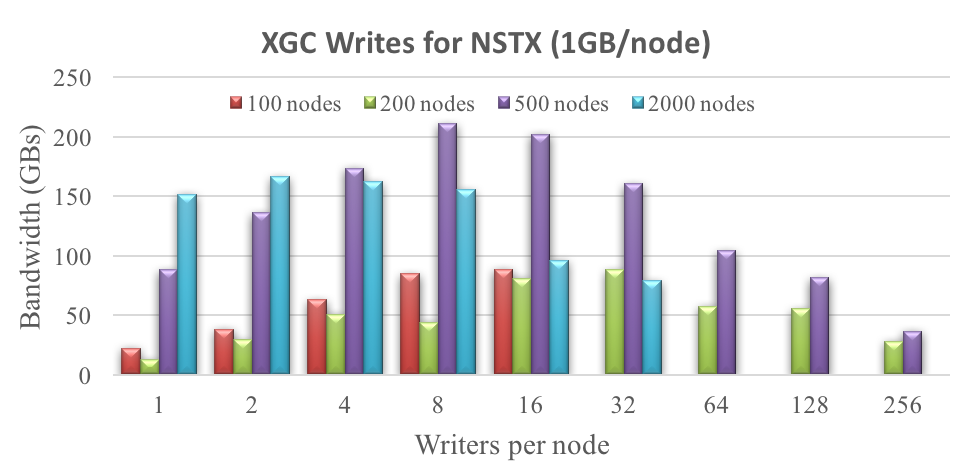
\includegraphics[width=0.45\textwidth]{figures/xgc_knl_cori.png}
\caption{Performance of the XGC application on Cori using KNL CPUs writing directly to the Lustre parallel file system. Experiments utilized a maximum of 200 OSTs. Optimal performance is obtained by having more writers per node for smaller node counts, whereas fewer writers per node perform well for larger allocations.}
\label{fig:XgcKnlCori}
\end{wrapfigure}

\section{Optimizing I/O through the use of Burst Buffers}
\label{chapter-bb}

We have some experience on using the new Burst Buffer technology. In this chapter we give specific advice on how to use ADIOS to write and read temporary data in a burst buffer. Currently, ADIOS does not have any "write-through" solution to use the burst buffer as caching, while storing data on a permanent file system. Rather, ADIOS supports scenarios where one wants just to write and read temporary data fast. Draining data from the burst buffer to a permanent storage is the user's task at the moment. Future ADIOS releases will utilize upcoming draining technologies to do this automatically. 

There are two different approaches to burst buffers. One is built of local fast storage on compute nodes, where one can only read data which is locally available. The other one is a parallel file system built of fast SSDs, that behave just like permanent parallel file systems with two limitations: total size, and the amount of data allowed to be written in a day. 

\subsection{Summit@OLCF}

The future Summit supercomputer at OLCF will have a Non-Volatile Memory (NVMe) storage device on each compute node. One can use ADIOS in scenarios where temporary data is written and read back later. For example, simulations with forward then backward simulation phases can store the outputs in the burst buffer and then read back the data backwards. Another example is checkpointing. Checkpoint data can be written (regularly) provided the job script drains the last checkpoint to the permanent storage. 

Our performance testing revealed that the best use of the burst buffer on Summit is to just write from every MPI task directly. That is, use the ADIOS POSIX transport for output to produce one file per MPI task. Unlike using a parallel file system (e.g., Lustre), files written to Burst Buffers on Summit will not be shareable between nodes. Files in Burst Buffers are only visible to the processes on the same node. For this reason, a special parameter for this transport (and for the \verb+MPI_AGGREGATE+ transport) is required: \verb+local-fs=1+ will make sure that every compute node will create the own output directory for the individual files. 

\begin{lstlisting}[language=XML]
<transport group="writer" method="POSIX">local-fs=1</transport>
\end{lstlisting}

At reading time, every process must only read data which had been written on the local node, otherwise zero-filled arrays will be returned. ADIOS can open the \verb+.bp+ file, which resides on the compute node where \verb+rank 0+ of the MPI application was writing the data, and distribute the metadata to every process. Thus, every process sees the global array definition but that does not mean it can read any piece of data. ADIOS does not have currently any reading transport to read data across nodes. 

\begin{figure}[h]
\center
\subfloat[ADIOS Write]{
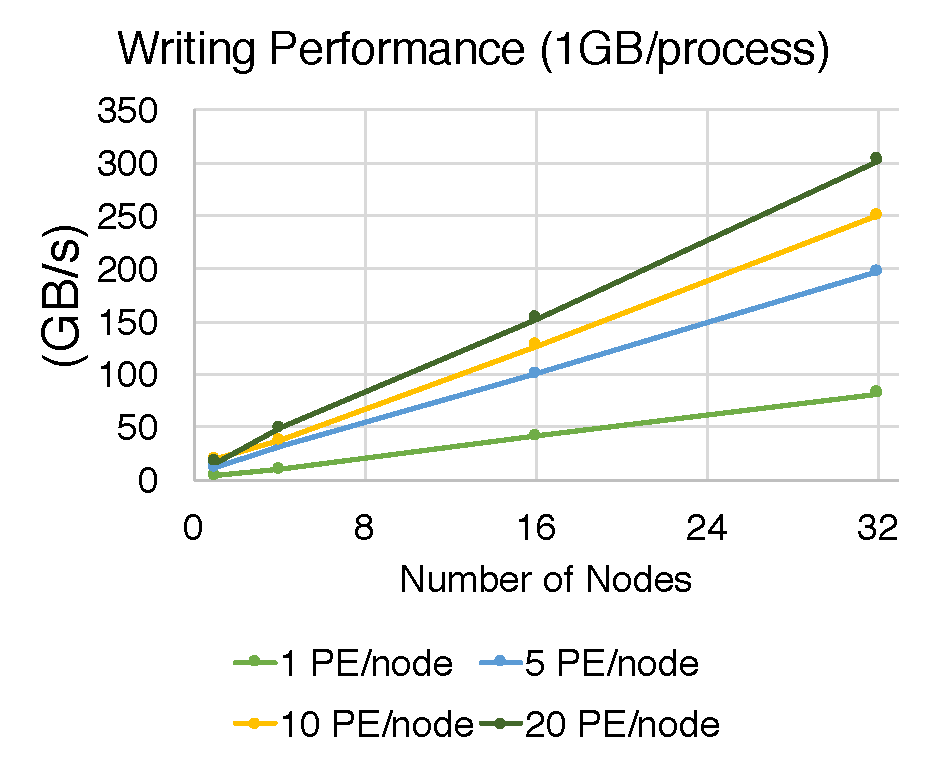
\includegraphics[width=0.33\textwidth]{figures/Adios_write_on_Summitdev.pdf}
\label{fig:summit_write}
}
\subfloat[ADIOS Read]{
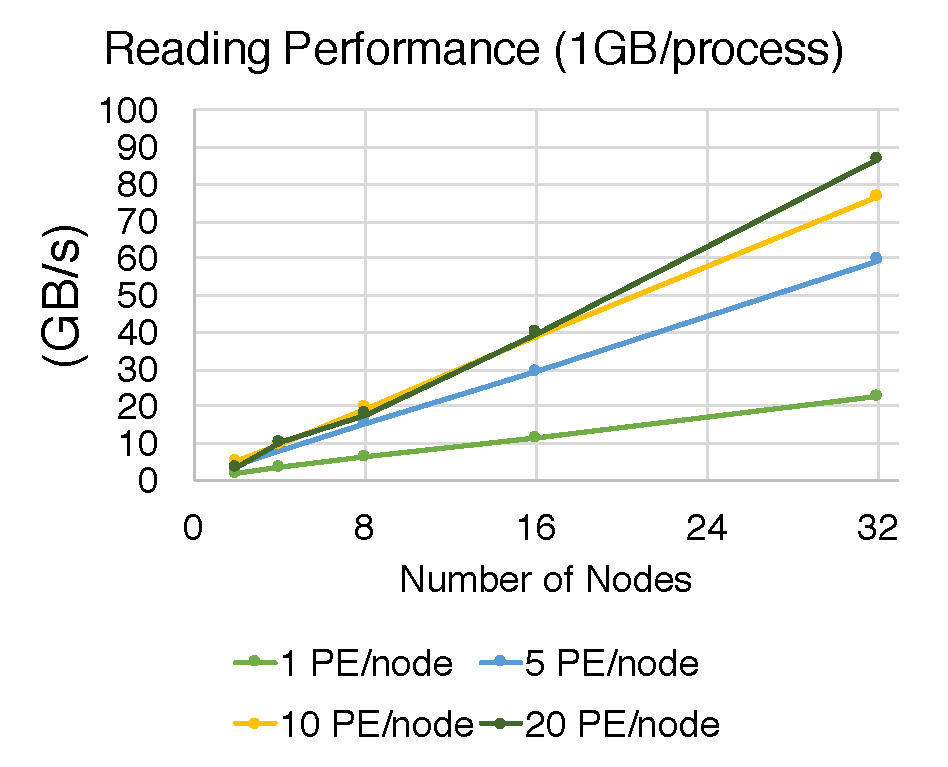
\includegraphics[width=0.33\textwidth]{figures/Adios_read_on_Summitdev.pdf}
\label{fig:summit_read}
}
\subfloat[Writing with no system cache]{
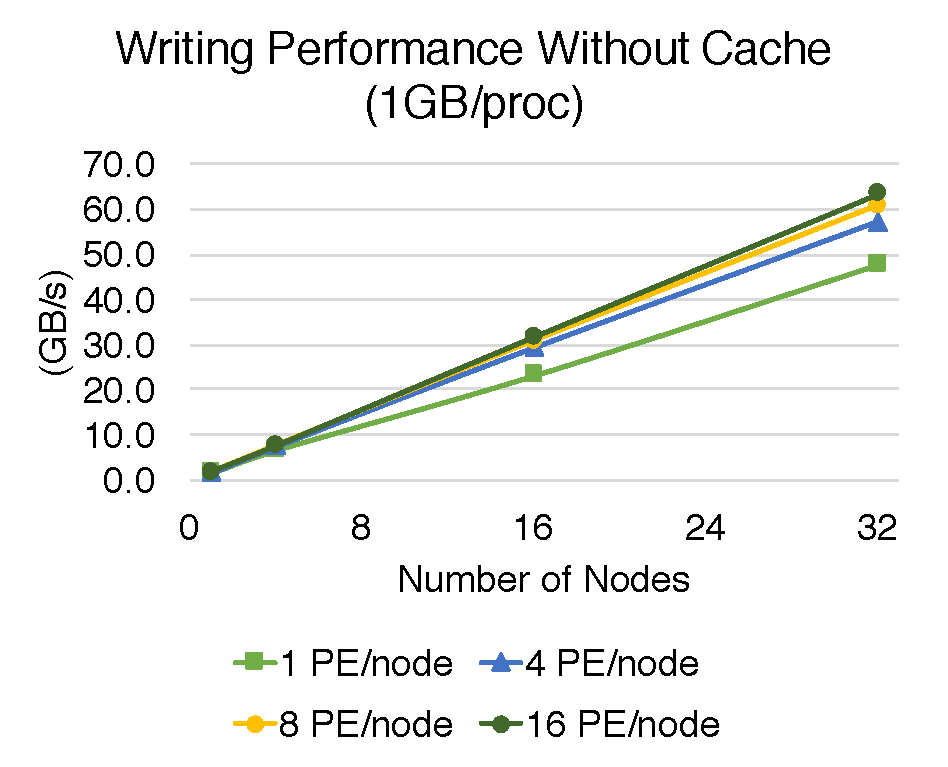
\includegraphics[width=0.33\textwidth]{figures/Adios_write_nocache_on_Summitdev.pdf}
\label{fig:summit_read}
}
\caption{ADIOS performance of (a) writing and (b) reading with Burst Buffer on Summit-dev (Summit's early access system) as of Jun 2017. Summit-dev has node-local NVMes. Note that the writing is accelerated by system cache, while reading I/O is not. Without system cache effect, we observed the write performance in (c)}
\label{fig:summit}
\end{figure}

Fig. ~\ref{fig:summit} shows some performance result on Summit measured in June 2017. We tried to assess the ADIOS write/read performance by writing/reading 1 GB data per process. We used different number of processes (1, 5, 10, and 20 processes) per node over different number of parallel nodes, ranging from 1 up to 32 nodes. Since Burst Buffers are node-local, we were able to achieve almost linear performance on writing and reading.  Note that writing performance is about 3.3x times better than reading in these tests. Writing performance is even better than the theoretically best raw throughput to the NVMe. This is because writing I/O is accelerated by system cache, while reading I/O is not. Without the system caching effect we could achieve up to 65 GB/s in similar application set-ups. This latter test was measured by using raw POSIX APIs with \verb+O_DIRECT+ option, not ADIOS.

\subsection{Cori@NERSC}

Unlike node-local NVMes on Summit, the Cori system has a centralized global parallel file system built from SSDs. Any compute node has access to the whole burst buffer and therefore it is somewhat easier to use it for storing temporary data. A user can copy the data after job termination to the disk based parallel file system (but before the data is purged according to NERSC policy).

\begin{wrapfigure}{l}{0.5\textwidth}
\center
%\subfloat[]{
\includegraphics[width=0.45\textwidth]{figures/Adios_write_on_Cori.pdf}
%\label{fig:summit_write}
%}
\caption{ADIOS performance with Burst Buffer on Cori as of Jun 2017. Cori has a centralized global parallel file system, called Burst Buffer.}
\label{fig:cori}
\end{wrapfigure}

Here is our recommendation on how to configure ADIOS for writing to the burst buffer on Cori.
As shown in \ref{fig:cori}, we measured ADIOS writing performance on Cori's KNL nodes with POSIX method. Across different number of writers (4, 16, 64, and 256) per compute node, we achieved the best performance with 16 writers per node. Although there are many different factors to consider, we recommend, in general, not to use too many writers (e.g., 256 writers) or too small number of writers (e.g, 4) per node with Burst Buffer.

Applications that use all cores on KNL nodes for MPI tasks, should consider using the \verb+MPI_AGGREGATE+ transport method. One can specify the number of processes that actually write to the file system with the \verb+num_aggregators+ option. Also use the \verb+striping=0+ option to use with Burst Buffer on Cori. 

For an example, if the application runs on 100 compute nodes, the following transport settings in the XML configuration file maintains 16 writers per node to write to the Burst Buffer:
\begin{lstlisting}[language=XML]
<transport group="writer" 
	method="MPI_AGGREGATE">num_aggregators=1600;striping=0;</transport>
\end{lstlisting}





\input{appendix}

\end{document}





